\documentclass[12pt]{beamer}
\usepackage{listings}
\usepackage[]{color}
\beamertemplatenavigationsymbolsempty
\AtBeginSection[]
{
    \begin{frame}
    \frametitle{Table of Contents}
    \tableofcontents[currentsection]
    \end{frame}
}
\lstset{language=C++, basicstyle=\footnotesize}
\setlength{\tabcolsep}{10pt}
\newcommand{\bigoh}{\mathcal{O}}

\title{Segment Tree and Lazy Propagation}
% \subtitle{DFS, BFS, applications}
\author{beOI Training}
\institute{
\includegraphics[height=12em]{../share/beoi-logo}}

\begin{document}

\frame{\titlepage}

\section{Regular Segment Tree}

\begin{frame}

\frametitle{Motivating problem}

You are given an integer array $A$ of size $n$ ($n < 10^6$).\\
Given two integers $a$ and $b$, can you give the minimum value of $A$ between indices $a$ and $b$ ?
\[
    \min_{i = a\ldots b} A[i]
\]

Well that's easy, just iterate over the interval and return the minimum!

\end{frame}

\begin{frame}

\frametitle{Motivating problem}

You are given an integer array $A$ of size $n$ ($n < 10^6$).\\
Given two integers $a$ and $b$, can you give give the minimum value of $A$ between indices $a$ and $b$ ?
\[
    \min_{i = a\ldots b} A[i]
\]

\begin{center}
\huge{100000 times?} 
\end{center}

This is called the \textbf{range minimum query} (RMQ) problem.

\end{frame}

\begin{frame}
    \frametitle{Naive solution}
    For each query, iterate over the corresponding range and return the minimum. \\
    If $k$ is the number of queries, time complexity is $\bigoh(nk)$. \\
    \textcolor{blue}{TLE}
\end{frame}

\begin{frame}
    \frametitle{Array representation of a binary tree}
    \begin{itemize}
        \item 1-based array, index 1 = root
        \item For each node of index $p$,
        \begin{itemize}
            \item left child has index $2p$
            \item right child has index $2p+1$
        \end{itemize}
    \end{itemize}
    \begin{center}
        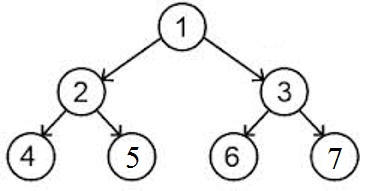
\includegraphics[width=.5\textwidth]{img/compact-array.jpg}
    \end{center}
\end{frame}

\begin{frame}
    \frametitle{Segment Tree}
    Each node is responsible of one segment \\
    Root represents the whole array $[0\cdots n-1]$ \\
    Given a node representing segment $[l\cdots r]$ 
    \begin{itemize}
        \item left child represents the segment's first half $\left[ l \cdots \frac{l+r}{2} \right]$
        \item right child represents the segment's second half $\left[ \frac{l+r}{2}+1\cdots r \right]$
    \end{itemize}
    The value of a node will be the \textbf{index of the minimum element in segment $\left[ l\cdots r \right]$}.

\end{frame}

\begin{frame}
    \frametitle{Querying}
    When we query the minimum value in an interval, we look for \textbf{big segments that are contained within the query range}, and among those segments, take the minimum value. \\
    Recursively,
    \begin{itemize}
        \item segment is within query range $\Rightarrow$ return value of the node;
        \item segment and query range are disjoint $\Rightarrow$ do nothing;
        \item otherwise, return minimum among both children.
    \end{itemize}
\end{frame}

\begin{frame}
    \frametitle{Querying implementation}

    \lstinputlisting{listings/query.cpp}
\end{frame}

\begin{frame}
    \frametitle{Querying complexity}

    At each level, at most 4 nodes are visited (see coach for proof). \\
    There are exactly $\lceil \log_2 n \rceil$ levels.
    \[
        \bigoh(4\times \lceil \log_2 n \rceil) = \bigoh(\log n)
    \]
    Overall complexity $\bigoh(k \log n)$ is now reasonable! \\
    \textcolor{green}{AC}
\end{frame}

\begin{frame}
    \frametitle{Building}
    Building the Segment Tree is also done recursively. \\
    For each node,
    \begin{itemize}
        \item if no child, store current index;
        \item otherwise,
            \begin{itemize}
                \item build left child;
                \item build right child;
                \item store minimum child.
            \end{itemize}
    \end{itemize}
\end{frame}

\begin{frame}
    \frametitle{Building implementation}
    \lstinputlisting{listings/build.cpp}
\end{frame}

\begin{frame}
    \frametitle{Building complexity}
    We visit every node once. \\
    In general, the number of nodes is $ N + \frac{N}{2} + \frac{N}{4} + \cdots + 2 + 1 \approx 2N $, so time complexity is
    \[ \bigoh(2\times N) = \bigoh(N) \]
    This also proves memory is $ \bigoh(N) $ (in practice one always takes an array of $4\times N$ for safety).
\end{frame}

\begin{frame}
    \frametitle{Segment Trees are extremely powerful!}
    We saw how to solve the range \textbf{minimum} query problem.\\
    But we can do much more than that! \\
    \begin{itemize}
        \item Range maximum query 
        \item Range sum query 
        \item Range *insert any function here* query
    \end{itemize}
\end{frame}

\begin{frame}
    \frametitle{One last operation}
    Suppose that, between queries, the array is being \textbf{updated}.\\
    Naive solution: re-build the Segment Tree in $ \bigoh(N) $. \\
    \textcolor{blue}{TLE} \\
    Segment Trees allow efficient \textbf{updating}!
\end{frame}

\begin{frame}
    \frametitle{Updating}
    To update $p$, we only need to update the segments that contain $p$. \\
    Update the leaf to root path in $ \bigoh(\log N) $!
\end{frame}

\begin{frame}
    \frametitle{Updating implementation}
    \lstinputlisting{listings/update.cpp}
\end{frame}

\section{Lazy Segment Tree}

\begin{frame}
    \frametitle{Motivating problem}
    In the Range Sum Query (RSQ) problem, we add one operation: range update. \\
    We want to update a range (e.g. increment every value in range by $k$) efficiently.
\end{frame}

\begin{frame}
    \frametitle{Naive solution}
    At each range update query, re-build tree in $\bigoh(N)$. \\
    \textcolor{blue}{TLE}
\end{frame}

\begin{frame}
    \frametitle{Let's be lazy!}
    Key idea behind lazy Segment Tree: don't update everything at once; put a flag on segments that need to be updated, and leave it for another traversal. \\
\end{frame}

\begin{frame}
    \frametitle{Propagation}
    Keep an array \lstinline{lazy} that stores for each segment by how much each value needs to be incremented. \\
    Every time we visit a node $p$ (in \lstinline{query} or \lstinline{update}) where \lstinline{lazy[p] != 0},
    \begin{itemize}
        \item increment current segment by \lstinline{lazy[p]} times size of segment;
        \item if node is not leaf,
            \begin{itemize}
                \item increment \lstinline{lazy[2*p]} by \lstinline{lazy[p]}
                \item increment \lstinline{lazy[2*p+1]} by \lstinline{lazy[p]}
            \end{itemize}
        \item reset \lstinline{lazy[p]}.
    \end{itemize}
    That is called \textbf{propagation}. \\
    Obviously, complexity is $\bigoh(1)$.
\end{frame}

\begin{frame}
    \frametitle{Propagation implementation}
    \lstinputlisting{listings/propagation.cpp}
\end{frame}

\begin{frame}
    \frametitle{Querying}
    We do exactly the same, but we propagate at each node! \\
    Complexity $\bigoh(\log N)$.

\end{frame}

\begin{frame}
    \frametitle{Querying implementation}
    \lstinputlisting{listings/lazy-query.cpp}
\end{frame}

\begin{frame}
    \frametitle{Updating}
    For each node, 
    \begin{itemize}
        \item propagate
        \item if outside of range, return
        \item if inside of range, set the lazy flag, and return
        \item otherwise
            \begin{itemize}
                \item update left child
                \item update right child
            \end{itemize}
        \item merge both children (add them up)
    \end{itemize}
    Complexity $\bigoh(\log N)$.
\end{frame}

\begin{frame}
    \frametitle{Updating implementation}
    \lstinputlisting{listings/lazy-update.cpp}
\end{frame}


\end{document}
